\begin{table*}[!t]
\centering
\caption{Hypothesis and Prediction Tests at $Q = 200$ (Recent Recall@10 Paired Gaps with \RNumCIPct{} CIs; H: hypothesis; PR: prediction; GT: gate; LK: look-ahead/underspend; Ref.: best refresh; DC: data-change; RN: recovered-neighbor; ES/ESO: batch/online extra search; PV: vector push; NR: never refresh; AF: always fresh; $^{\ast}$lead or tie weakens or disappears when data-change's score messages are charged, Table~\ref{tab:add3}). H4/H4b pass if refresh beats both alternatives (3-way gaps in Table~\ref{tab:m2_m3_equal_bytes}).}
\label{tab:hypotheses}
\scriptsize
\renewcommand{\arraystretch}{0.68}
\setlength{\tabcolsep}{1.0pt}
\begin{tabular}{@{}lllll@{}}
\toprule
\textbf{Test} & \textbf{Comparison ($Q{=}200$)} & \textbf{Steady Stream} & \textbf{New-Topic Stream} & \textbf{Outcome (Steady / New-Topic)} \\
\midrule
H1 & M1 AF $-$ NR ($B{=}4$) & \RNumHOneGapSteady{} & \RNumHOneGapNewTopic{} & Pass / Pass (means and upper CIs $< {}$\RNumGateThresholdPP{}) \\
H2 & M1 ES $-$ Ref.\ ($B{=}4$) & \RNumHTwoESvsRefreshSteady{} & \RNumHTwoESvsRefreshNewTopic{} & Pass / Pass \\
 & M1 PV $-$ Ref.\ ($B{=}4$) & \RNumHTwoPVvsRefreshSteady{} & \RNumHTwoPVvsRefreshNewTopic{} & Pass / Pass \\
H2b & M1 ESO $-$ Ref.\ ($B{=}4$) & \RNumHTwoBESOvsRefreshSteady{} & \RNumHTwoBESOvsRefreshNewTopic{} & Pass / Pass \\
PR2 & M2 $5$ rules $-$ AF (all $B$) & \RNumPredMTwoTiesGap{} & \RNumPredMTwoTiesGap{} & Pass / Pass (exact tie; max diff \RNumPredMTwoTiesMaxAbs{}) \\
GT2 & M2 AF $-$ NR ($B{=}4$) & \RNumGateMTwoSteady{} & \RNumGateMTwoNewTopic{} & Fail ($< {}$\RNumGateThresholdPP{}) / Pass ($\ge {}$\RNumGateThresholdPP{}) \\
H3 & M2 RN $-$ other $4$ ($B{=}4$) & \RNumHThreeGapZero{} & \RNumHThreeGapZero{} & Gated / Fail (tie by construction) \\
H4 & M2 Ref.\ $-$ PV ($B{=}2$) & \RNumHFourRefMinusPVBTwoSteady{} & \RNumHFourRefMinusPVBTwoNewTopic{} & Fail (PV wins) / Pass (Refresh wins) \\
 & M2 Ref.\ $-$ PV ($B{=}4$) & \RNumHFourRefMinusPVBFourSteady{} & \RNumHFourRefMinusPVBFourNewTopic{} & Fail (PV wins) / Pass (Refresh wins) \\
 & M2 Ref.\ $-$ PV ($B{=}8$) & \RNumHFourRefMinusPVBEightSteady{} & \RNumHFourRefMinusPVBEightNewTopic{} & Fail (PV wins) / Pass (Refresh wins) \\
PR3 & M3 $4$ rules $-$ AF ($B{=}8$) & \RNumPredMThreeBEightFourRulesGap{} & \RNumPredMThreeBEightFourRulesGap{} & Pass / Pass (exact tie; max diff \RNumPredMThreeBEightFourRulesMaxAbs{})$^{\ast}$ \\
 & M3 RN $-$ AF ($B{=}8$) & \RNumPredMThreeBEightRNGapSteady{} & \RNumPredMThreeBEightRNGapNewTopic{} & \begin{tabular}[t]{@{}l@{}}Not predicted to tie (means shown; max per-query\\recall difference \RNumPredMThreeBEightRNMaxAbsOne{} on single-recent-neighbor queries)\end{tabular} \\
GT3 & M3 AF $-$ NR ($B{=}4$) & \RNumGateMThreeSteady{} & \RNumGateMThreeNewTopic{} & Fail ($< {}$\RNumGateThresholdPP{}) / Pass ($\ge {}$\RNumGateThresholdPP{}) \\
H3b & M3 RN $-$ DC ($B{=}4$) & \RNumHThreeBRNMinusDCSteady{} & \RNumHThreeBRNMinusDCNewTopic{} & Gated / Fail (data-change wins)$^{\ast}$ \\
H4b & M3 Ref.\ $-$ PV ($B{=}2$) & \RNumHFourBRefMinusPVBTwoSteady{} & \RNumHFourBRefMinusPVBTwoNewTopic{} & Fail (PV wins) / Pass, fragile (refresh ahead)$^{\ast}$ \\
 & M3 Ref.\ $-$ PV ($B{=}4$) & \RNumHFourBRefMinusPVBFourSteady{} & \RNumHFourBRefMinusPVBFourNewTopic{} & Fail (PV wins) / Fail (no clear winner)$^{\ast}$ \\
 & M3 Ref.\ $-$ PV ($B{=}8$) & \RNumHFourBRefMinusPVBEightSteady{} & \RNumHFourBRefMinusPVBEightNewTopic{} & Fail (PV wins) / Fail (PV wins) \\
LK & M1 ES $-$ ESO ($B{=}4$) & \RNumLookaheadMOneQTwoHundredSteady{} & \RNumLookaheadMOneQTwoHundredNewTopic{} & Small at $Q = 200$ ($\le {}$\RNumLookaheadMOneMaxQTwoHundred{}) \\
 & M3 ES $-$ ESO ($B{=}4$) & \RNumLookaheadMThreeBFourSteady{} & \RNumLookaheadMThreeBFourNewTopic{} & Small at $Q = 200$ ($\le {}$\RNumLookaheadMThreeMaxBFour{}) \\
\bottomrule
\end{tabular}
\end{table*}

\section{Experimental Results}
\label{sec:results}

In all $5$ main suites (\RNumTotalMainRuns{} runs, \RNumMissingRuns{} missing) and Exploratory Addendum 3 (\RNumAddThreeTotalRuns{} runs; \RNumAddThreeMThreeFailedAttempts{}/\RNumAddThreeMThreeRuns{} M3 runs retried OK after a first-attempt memory error), every run finished and spent $\le B$ on charged messages (uncharged costs in Section~\ref{sec:system}). Table~\ref{tab:hypotheses} lists every registered test. At $Q{=}200$ (\RNumQueriesPerSeedQTwoHundred{} queries/seed, \RNumNumEpochs{} epochs), recent recall@10 is defined on \RNumQueriesWithRecentSteadyQTwoHundred{}/\RNumQueriesTotalQTwoHundred{} steady (\RNumQueriesWithRecentFracSteadyQTwoHundred{}) and \RNumQueriesWithRecentNewTopicQTwoHundred{}/\RNumQueriesTotalQTwoHundred{} new-topic queries (\RNumQueriesWithRecentFracNewTopicQTwoHundred{}, \RNumNewTopicValidQueriesSeedMinQTwoHundred{} to \RNumNewTopicValidQueriesSeedMaxQTwoHundred{}/seed; at $Q \in \{50, 800\}$: \RNumQueriesWithRecentSteadyQFifty{}, \RNumQueriesWithRecentSteadyQEightHundred{} steady; \RNumQueriesWithRecentNewTopicQFifty{}, \RNumQueriesWithRecentNewTopicQEightHundred{} new-topic).\looseness=-1

\subsection{Centroid Placement (M1 and M1-Online)}
\label{sec:results_m1}

\textbf{Small fresh-summary headroom (H1).} Under centroid placement ($Q = 200, B = 4$), each arrival joins the shard with the nearest initial centroid, so setup summaries already steer queries to new arrivals. Refreshing all \RNumNumShards{} summaries (\RNumAlwaysFreshEpochBytes{} B/epoch) changes recent recall@10 from \RNumMOneNRRecentSteady{} (never refresh) to \RNumMOneAFRecentSteady{} on steady (\RNumHOneGapSteady{}, not significant) and from \RNumMOneNRRecentNewTopic{} to \RNumMOneAFRecentNewTopic{} on new-topic (\RNumHOneGapNewTopic{}). Both upper \RNumCIPct{} bounds sit below \RNumGateThresholdPP{}, confirming H1 across seeds \RNumSeedMin{} to \RNumSeedMax{} (with pilot seed \RNumPilotSeed{}). On out-of-sample seeds \RNumOutOfSampleSeedMin{} to \RNumSeedMax{}, pooled/unweighted means are \RNumHOneOutOfSampleMeanSteady{} and \RNumHOneOutOfSampleUnweightedMeanSteady{} (\RNumHOneOutOfSampleMinSteady{} to \RNumHOneOutOfSampleMaxSteady{}) on steady and \RNumHOneOutOfSampleMeanNewTopic{} and \RNumHOneOutOfSampleUnweightedMeanNewTopic{} (\RNumHOneOutOfSampleMinNewTopic{} to \RNumHOneOutOfSampleMaxNewTopic{}) on new-topic. Overall recall@10 changes by \RNumHOneOverallGapSteady{} on steady and \RNumHOneOverallGapNewTopic{} on new-topic. Against $m{=}2$ oracle routing, which picks the two shards holding the most overall top-$10$ neighbors (\RNumMOneOracleRecentSteady{} steady, \RNumMOneOracleRecentNewTopic{} new-topic; all-shard \RNumMOneAllShardsRecentSteady{}, \RNumMOneAllShardsRecentNewTopic{}), full refresh closes only \RNumMOneAFShareOfOracleSteady{} and \RNumMOneAFShareOfOracleNewTopic{} of the never-refresh-to-oracle gap.\looseness=-1

\textbf{Equal-byte alternatives at $Q = 200$ (H2 and H2b).} Over \RNumNumEpochs{} epochs at $B{=}4$ (\RNumBudgetBFourEpochBytes{} B/epoch), four refresh rules spend \RNumMOneFourRulesBytes{} B, RN spends \RNumMOneRNBytes{} B (\RNumMOneRNAmortBytes{} amortized), ES spends \RNumMOneESBytes{} B, ESO spends \RNumMOneESOBytesSteady{} (steady) and \RNumMOneESOBytesNewTopic{} (new-topic; \RNumMOneESOShareOfESQTwoHundredSteady{} and \RNumMOneESOShareOfESQTwoHundredNewTopic{} of ES), and PV spends \RNumMOnePVBytes{} B (\RNumMOnePVPushedVecs{} vectors). Refresh rules span \RNumMOneRRRecentMeanSteady{} (RR) to \RNumMOneRNRecentMeanSteady{} (RN, best; none beats NR reliably) on steady and \RNumMOneRRRecentMeanNewTopic{} (RR) to \RNumMOneDCRecentMeanNewTopic{} (DC, best) on new-topic. At equal bytes, ES (\RNumMOneESRecentSteady{}, \RNumMOneESRecentNewTopic{}), ESO (\RNumMOneESORecentSteady{}, \RNumMOneESORecentNewTopic{}), and PV (\RNumMOnePVRecentSteady{}, \RNumMOnePVRecentNewTopic{}) all beat best refresh. On steady, their gains over best refresh are \RNumHTwoESvsRefreshSteady{}, \RNumHTwoBESOvsRefreshSteady{}, and \RNumHTwoPVvsRefreshSteady{}. On new-topic, they are \RNumHTwoESvsRefreshNewTopic{}, \RNumHTwoBESOvsRefreshNewTopic{}, and \RNumHTwoPVvsRefreshNewTopic{} (H2 and H2b pass; all three beat every refresh rule, and batch extra search and vector push beat always-fresh). On out-of-sample seeds \RNumOutOfSampleSeedMin{} to \RNumSeedMax{}, every per-seed ES and PV gain over best refresh is positive. Probing a third shard on $\le {}$\RNumExtraSearchesBFour{} close-margin queries/epoch (\RNumESLoadPctQTwoHundred{} shard load at $Q{=}200$, \RNumThreeShards{}-shard fan-out or extra round trip) improves general routing. It raises overall recall@10 over best refresh by \RNumHTwoESvsRefreshOverallSteady{} and \RNumHTwoBESOvsRefreshOverallSteady{} on steady and \RNumHTwoESvsRefreshOverallNewTopic{} and \RNumHTwoBESOvsRefreshOverallNewTopic{} on new-topic. Vector push is a sampling effect: buffering \RNumMOnePVPushedVecs{}/\RNumSteadyStreamTotalVecs{} streamed vectors (\RNumMOnePVShareSteady{}, $p = {}$\RNumMOnePVShareFracSteady{}) predicts $R_{\text{NR}} + p(1 - R_{\text{NR}}) = {}$\RNumMOnePVPredRecentSteady{} on steady from never-refresh $R_{\text{NR}}$ (observed \RNumMOnePVRecentSteady{}; $p$ falls as inserts grow; summary size is fixed). It raises overall recall@10 over best refresh by only \RNumHTwoPVvsRefreshOverallSteady{} (steady) and \RNumHTwoPVvsRefreshOverallNewTopic{} (new-topic), scanning $\le {}$\RNumPVMaxVecsBFour{} vectors in coordinator memory (\RNumPVFifoVecsBFour{} FIFO vectors suffice for recent recall@10).\looseness=-1

\begin{table}[!t]
\centering
\caption{Centroid Query-Rate Sweep at $B = 4$ (Recent Recall@10 Gaps in pp, \RNumCIPct{} CIs; Ref.: best $Q{=}200$ refresh, recovered-neighbor on steady, data-change on new-topic; ES/ESO: batch/online extra search; PV: vector push; gaps are Ref.\ $-$ alt., opposite to H2/H2b in Table~\ref{tab:hypotheses}; $^{\ast}$lead or tie weakens or disappears when data-change's score messages are charged, Table~\ref{tab:add3}).}
\label{tab:q_sweep}
\scriptsize
\renewcommand{\arraystretch}{0.68}
\setlength{\tabcolsep}{3.0pt}
\begin{tabular}{@{}llll@{}}
\toprule
\textbf{$Q$} & \textbf{Comp.} & \textbf{Steady Stream (pp)} & \textbf{New-Topic Stream (pp)} \\
\midrule
$50$ & Ref.\ $-$ ES & \RNumQSweepRefMinusESQFiftySteadyCell{} & \RNumQSweepRefMinusESQFiftyNewTopicCell{} \\
 & Ref.\ $-$ ESO & \RNumQSweepRefMinusESOQFiftySteadyCell{} & \RNumQSweepRefMinusESOQFiftyNewTopicCell{} \\
 & Ref.\ $-$ PV & \RNumQSweepRefMinusPVQFiftySteadyCell{} & \RNumQSweepRefMinusPVQFiftyNewTopicCell{} \\
 & ES $-$ ESO & \RNumLookaheadMOneQFiftySteadyCell{} & \RNumLookaheadMOneQFiftyNewTopicCell{} \\
$200$ & Ref.\ $-$ ES & \RNumQSweepRefMinusESQTwoHundredSteadyCell{} & \RNumQSweepRefMinusESQTwoHundredNewTopicCell{} \\
 & Ref.\ $-$ ESO & \RNumQSweepRefMinusESOQTwoHundredSteadyCell{} & \RNumQSweepRefMinusESOQTwoHundredNewTopicCell{} \\
 & Ref.\ $-$ PV & \RNumQSweepRefMinusPVQTwoHundredSteadyCell{} & \RNumQSweepRefMinusPVQTwoHundredNewTopicCell{} \\
 & ES $-$ ESO & \RNumLookaheadMOneQTwoHundredSteadyCell{} & \RNumLookaheadMOneQTwoHundredNewTopicCell{} \\
$800$ & Ref.\ $-$ ES & \RNumQSweepRefMinusESQEightHundredSteadyCell{} & \RNumQSweepRefMinusESQEightHundredNewTopicCell{}$^{\ast}$ \\
 & Ref.\ $-$ ESO & \RNumQSweepRefMinusESOQEightHundredSteadyCell{} & \RNumQSweepRefMinusESOQEightHundredNewTopicCell{}$^{\ast}$ \\
 & Ref.\ $-$ PV & \RNumQSweepRefMinusPVQEightHundredSteadyCell{} & \RNumQSweepRefMinusPVQEightHundredNewTopicCell{} \\
 & ES $-$ ESO & \RNumLookaheadMOneQEightHundredSteadyCell{} & \RNumLookaheadMOneQEightHundredNewTopicCell{} \\
\bottomrule
\end{tabular}
\end{table}

\begin{table}[!t]
\centering
\caption{Arrival-Time Equal-Byte Comparisons ($Q{=}200$, Recent Recall@10 Gaps in pp, \RNumCIPct{} CIs; Ref.: best refresh per $B$, M2 $5$ tie AF, M3 SS at $B{=}2$ steady, DC at $B{=}4$ steady and $B{\le}4$ new-topic, $4$ tie AF at $B{=}8$; ES/ESO: batch/online extra search; PV: vector push; SS: shard-size; DC: data-change; AF: always fresh; $^{\ast}$lead or tie weakens or disappears when data-change's score messages are charged, Table~\ref{tab:add3}).}
\label{tab:m2_m3_equal_bytes}
\scriptsize
\renewcommand{\arraystretch}{0.68}
\setlength{\tabcolsep}{3.0pt}
\begin{tabular}{@{}llll@{}}
\toprule
\textbf{ID ($B$)} & \textbf{Comp.} & \textbf{Steady Stream (pp)} & \textbf{New-Topic Stream (pp)} \\
\midrule
M2 ($2$) & Ref.\ $-$ ES & \RNumHFourRefMinusESBTwoSteadyCell{} & \RNumHFourRefMinusESBTwoNewTopicCell{} \\
 & Ref.\ $-$ PV & \RNumHFourRefMinusPVBTwoSteadyCell{} & \RNumHFourRefMinusPVBTwoNewTopicCell{} \\
 & ES $-$ PV & \RNumHFourESMinusPVBTwoSteadyCell{} & \RNumHFourESMinusPVBTwoNewTopicCell{} \\
M2 ($4$) & Ref.\ $-$ ES & \RNumHFourRefMinusESBFourSteadyCell{} & \RNumHFourRefMinusESBFourNewTopicCell{} \\
 & Ref.\ $-$ PV & \RNumHFourRefMinusPVBFourSteadyCell{} & \RNumHFourRefMinusPVBFourNewTopicCell{} \\
 & ES $-$ PV & \RNumHFourESMinusPVBFourSteadyCell{} & \RNumHFourESMinusPVBFourNewTopicCell{} \\
M2 ($8$) & Ref.\ $-$ ES & \RNumHFourRefMinusESBEightSteadyCell{} & \RNumHFourRefMinusESBEightNewTopicCell{} \\
 & Ref.\ $-$ PV & \RNumHFourRefMinusPVBEightSteadyCell{} & \RNumHFourRefMinusPVBEightNewTopicCell{} \\
 & ES $-$ PV & \RNumHFourESMinusPVBEightSteadyCell{} & \RNumHFourESMinusPVBEightNewTopicCell{} \\
M3 ($2$) & Ref.\ $-$ ESO & \RNumHFourBRefMinusESOBTwoSteadyCell{} & \RNumHFourBRefMinusESOBTwoNewTopicCell{}$^{\ast}$ \\
 & Ref.\ $-$ PV & \RNumHFourBRefMinusPVBTwoSteadyCell{} & \RNumHFourBRefMinusPVBTwoNewTopicCell{}$^{\ast}$ \\
 & ESO $-$ PV & \RNumHFourBESOMinusPVBTwoSteadyCell{} & \RNumHFourBESOMinusPVBTwoNewTopicCell{} \\
M3 ($4$) & Ref.\ $-$ ESO & \RNumHFourBRefMinusESOBFourSteadyCell{} & \RNumHFourBRefMinusESOBFourNewTopicCell{}$^{\ast}$ \\
 & Ref.\ $-$ PV & \RNumHFourBRefMinusPVBFourSteadyCell{} & \RNumHFourBRefMinusPVBFourNewTopicCell{}$^{\ast}$ \\
 & ESO $-$ PV & \RNumHFourBESOMinusPVBFourSteadyCell{} & \RNumHFourBESOMinusPVBFourNewTopicCell{} \\
M3 ($8$) & Ref.\ $-$ ESO & \RNumHFourBRefMinusESOBEightSteadyCell{} & \RNumHFourBRefMinusESOBEightNewTopicCell{} \\
 & Ref.\ $-$ PV & \RNumHFourBRefMinusPVBEightSteadyCell{} & \RNumHFourBRefMinusPVBEightNewTopicCell{} \\
 & ESO $-$ PV & \RNumHFourBESOMinusPVBEightSteadyCell{} & \RNumHFourBESOMinusPVBEightNewTopicCell{} \\
\bottomrule
\end{tabular}
\end{table}

\textbf{Query-rate sweep ($Q \in \{50, 200, 800\}$) and look-ahead.} Table~\ref{tab:q_sweep} varies $Q$ at $B = 4$, holding the $Q = 200$ refresh winner fixed across $Q$ (unlike Table~\ref{tab:m2_m3_equal_bytes}, which picks the best rule per $B$). On steady, recovered-neighbor (\RNumMOneRNRecentMeanQFiftySteady{}) trails data-change (\RNumMOneDCRecentMeanQFiftySteady{}) by \RNumMOneDCMinusRNQFiftySteady{} at $Q{=}50$ (DC minus PV: \RNumMOneDCMinusPVQFiftySteady{}). At $Q{=}800$, the five rules span only \RNumMOneRNRecentMeanQEightHundredSteady{} (RN) to \RNumMOneDCRecentMeanQEightHundredSteady{} (DC). Extra search and vector push beat every refresh rule at every $Q$ on steady (smallest gap, DC minus ESO at $Q{=}800$: \RNumMOneDCMinusESOQEightHundredSteady{}). Summary refresh and pushed vectors amortize across all queries, whereas $B = 4$ buys at most \RNumExtraSearchesBFour{} extra searches per epoch (\RNumESLoadPctQFifty{}, \RNumESLoadPctQTwoHundred{}, and \RNumESLoadPctQEightHundred{} shard load at $Q \in \{50, 200, 800\}$). On new-topic at $Q = 800$ with score bytes uncharged ($n_B = 4$), data-change refresh (\RNumQSweepRefRecentQEightHundredNewTopic{}) overtakes batch (\RNumQSweepESRecentQEightHundredNewTopic{}, by \RNumQSweepRefMinusESQEightHundredNewTopic{}) and online extra search (\RNumQSweepESORecentQEightHundredNewTopic{}, by \RNumQSweepRefMinusESOQEightHundredNewTopic{}). In Exploratory Addendum 3 (X4, $n_B{=}3$, Table~\ref{tab:add3}), charged data-change edges batch extra search on new-topic by only \RNumAddThreeXFourESNewTopic{} ($t$-interval \RNumAddThreeXFourESNewTopicTInt{}) and trails both extra searches on steady. That lead is fragile. Its lower CI bound is \RNumAddThreeXFourESNewTopicBootLow{} (touching zero under other bootstrap seeds), it comes from epochs $0$ to $29$ (\RNumAddThreeXFourESNewTopicEarlyMean{} vs.\ \RNumAddThreeXFourESNewTopicLateMean{} in epochs $30$ to $49$), and it is not ahead on overall recall@10 (\RNumAddThreeXFourESOverallNewTopic{}). Vector push (\RNumQSweepPVRecentQEightHundredNewTopic{} at $Q{=}800$) beats refresh on new-topic at every $Q$: uncharged refresh minus vector push is \RNumQSweepRefMinusPVQFiftyNewTopic{} at $Q{=}50$ ($t$-interval \RNumQSweepRefMinusPVQFiftyNewTopicTInt{}) and \RNumQSweepRefMinusPVQEightHundredNewTopic{} at $Q{=}800$ (charged: Table~\ref{tab:add3}). At $Q \ge 200$, LK (ES $-$ ESO in Table~\ref{tab:q_sweep}) is at most \RNumLookaheadMOneQTwoHundredSteady{} ($Q{=}200$ steady, $t$-interval \RNumLookaheadMOneQTwoHundredSteadyTInt{}, seed \RNumLookaheadMOneQTwoHundredSteadyNegSeed{} \RNumLookaheadMOneQTwoHundredSteadyNegSeedGap{}); on new-topic, ESO spends \RNumMOneESOShareOfESQTwoHundredNewTopic{} to \RNumMOneESOShareOfESQEightHundredNewTopic{} of ES bytes, mixing look-ahead with underspend. At $Q{=}50$, LK (\RNumLookaheadMOneQFiftySteady{} steady, \RNumLookaheadMOneQFiftyNewTopic{} new-topic) mixes look-ahead with per-query and byte caps. Online, by design, makes $\le 1$ search/query (\RNumESOQFiftyMaxSearches{}/epoch) and spends \RNumMOneESOShareOfESQFiftySteady{} and \RNumMOneESOShareOfESQFiftyNewTopic{} of batch bytes.\looseness=-1

\begin{figure}[!t]
\centering
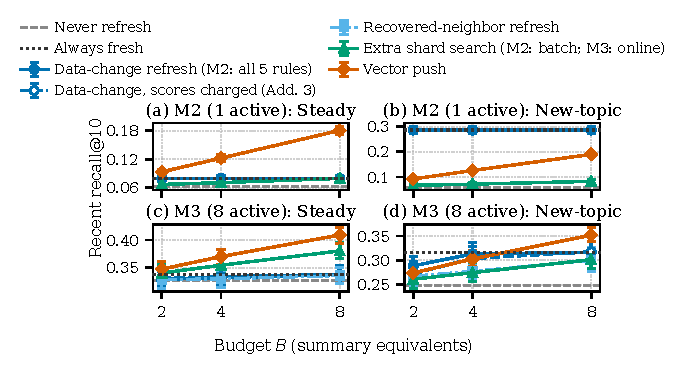
\includegraphics[width=\columnwidth]{figures/fig_m2_m3_budget.pdf}
\caption{Recent recall@10 across $B \in \{2, 4, 8\}$ at $Q{=}200$ in M2 (top, batch ES; all $5$ equal AF) and M3 (bottom, online ESO); y-axes differ. Dashed blue (c, d): data-change with its \RNumDCScoreEpochBytes{} B/epoch of score messages charged ($n_B \in \{1, 3, 7\}$; exploratory Addendum 3, M3 only). Error bars: unpaired per-method \RNumCIPct{} CIs, overlapping even where paired gaps in Table~\ref{tab:m2_m3_equal_bytes} exclude zero (Panel c, $B{=}2$: SS is \RNumMThreeSSMinusDCBTwoSteady{} above plotted DC).}
\label{fig:equal_bytes_b}
\end{figure}

\begin{table}[!t]
\centering
\caption{Refresh Rules and Baselines ($Q{=}200$, Recent Recall@10; St.: steady; NT: new-topic; NR: never refresh; RR: round-robin; DC: data-change; RN: recovered-neighbor; QL: query-popularity; SS: shard-size; AF: always fresh; M2 omitted: all $5$ tie AF; DC is the uncharged rule; charged gaps are in Table~\ref{tab:add3}).}
\label{tab:refresh_rules}
\scriptsize
\renewcommand{\arraystretch}{0.68}
\setlength{\tabcolsep}{1.6pt}
\begin{tabular}{@{}llccccccc@{}}
\toprule
\textbf{Cond.} & \textbf{Str.} & \textbf{NR} & \textbf{RR} & \textbf{DC} & \textbf{RN} & \textbf{QL} & \textbf{SS} & \textbf{AF} \\
\midrule
M1 ($B{=}4$) & St. & \RNumMOneNRRecentSteady{} & \RNumMOneRRRecentSteady{} & \RNumMOneDCRecentSteady{} & \RNumMOneRNRecentSteady{} & \RNumMOneQLRecentSteady{} & \RNumMOneSSRecentSteady{} & \RNumMOneAFRecentSteady{} \\
M3 ($B{=}2$) & St. & \RNumMThreeNRRecentSteady{} & \RNumMThreeRRRecentBTwoSteady{} & \RNumMThreeDCRecentBTwoSteady{} & \RNumMThreeRNRecentBTwoSteady{} & \RNumMThreeQLRecentBTwoSteady{} & \RNumMThreeSSRecentBTwoSteady{} & \RNumMThreeAFRecentSteady{} \\
M3 ($B{=}4$) & St. & \RNumMThreeNRRecentSteady{} & \RNumMThreeRRRecentBFourSteady{} & \RNumMThreeDCRecentBFourSteady{} & \RNumMThreeRNRecentBFourSteady{} & \RNumMThreeQLRecentBFourSteady{} & \RNumMThreeSSRecentBFourSteady{} & \RNumMThreeAFRecentSteady{} \\
M3 ($B{=}8$) & St. & \RNumMThreeNRRecentSteady{} & \RNumMThreeRRRecentBEightSteady{} & \RNumMThreeDCRecentBEightSteady{} & \RNumMThreeRNRecentBEightSteady{} & \RNumMThreeQLRecentBEightSteady{} & \RNumMThreeSSRecentBEightSteady{} & \RNumMThreeAFRecentSteady{} \\
M1 ($B{=}4$) & NT & \RNumMOneNRRecentNewTopic{} & \RNumMOneRRRecentNewTopic{} & \RNumMOneDCRecentNewTopic{} & \RNumMOneRNRecentNewTopic{} & \RNumMOneQLRecentNewTopic{} & \RNumMOneSSRecentNewTopic{} & \RNumMOneAFRecentNewTopic{} \\
M3 ($B{=}2$) & NT & \RNumMThreeNRRecentNewTopic{} & \RNumMThreeRRRecentBTwoNewTopic{} & \RNumMThreeDCRecentBTwoNewTopic{} & \RNumMThreeRNRecentBTwoNewTopic{} & \RNumMThreeQLRecentBTwoNewTopic{} & \RNumMThreeSSRecentBTwoNewTopic{} & \RNumMThreeAFRecentNewTopic{} \\
M3 ($B{=}4$) & NT & \RNumMThreeNRRecentNewTopic{} & \RNumMThreeRRRecentBFourNewTopic{} & \RNumMThreeDCRecentBFourNewTopic{} & \RNumMThreeRNRecentBFourNewTopic{} & \RNumMThreeQLRecentBFourNewTopic{} & \RNumMThreeSSRecentBFourNewTopic{} & \RNumMThreeAFRecentNewTopic{} \\
M3 ($B{=}8$) & NT & \RNumMThreeNRRecentNewTopic{} & \RNumMThreeRRRecentBEightNewTopic{} & \RNumMThreeDCRecentBEightNewTopic{} & \RNumMThreeRNRecentBEightNewTopic{} & \RNumMThreeQLRecentBEightNewTopic{} & \RNumMThreeSSRecentBEightNewTopic{} & \RNumMThreeAFRecentNewTopic{} \\
\bottomrule
\end{tabular}
\end{table}

\begin{table}[!t]
\centering
\caption{Exploratory Addendum 3: Charged Data-Change Minus Each Method (Recent Recall@10 Gaps in pp, \RNumCIPct{} CIs;
charged DC sends $n_B \in \{1, 3, 7\}$ summaries and leaves \RNumAddThreeDCUnspentEpochBytes{} B/epoch of $B$ unspent; X1: vs.\ RN at equal $n_B$; X2: vs.\ PV and ESO; X3: vs.\
uncharged DC; X4: M1, $Q{=}800$, $B{=}4$; ES/ESO: batch/online extra search; PV: vector push;
$^\dagger$fragile, see text).}
\label{tab:add3}
\scriptsize
\renewcommand{\arraystretch}{0.68}
\setlength{\tabcolsep}{3.0pt}
\begin{tabular}{@{}llll@{}}
\toprule
Set ($B$) & Minus & Steady Stream (pp) & New-Topic Stream (pp) \\
\midrule
M3 ($2$) & X1 RN & \RNumAddThreeXOneRNBTwoSteadyCell{} & \RNumAddThreeXOneRNBTwoNewTopicCell{} \\
         & X2 PV & \RNumAddThreeXTwoPVBTwoSteadyCell{} & \RNumAddThreeXTwoPVBTwoNewTopicCell{} \\
         & X2 ESO & \RNumAddThreeXTwoESOBTwoSteadyCell{} & \RNumAddThreeXTwoESOBTwoNewTopicCell{} \\
         & X3 DC & \RNumAddThreeXThreeDCBTwoSteadyCell{} & \RNumAddThreeXThreeDCBTwoNewTopicCell{}$^\dagger$ \\
M3 ($4$) & X1 RN & \RNumAddThreeXOneRNBFourSteadyCell{} & \RNumAddThreeXOneRNBFourNewTopicCell{} \\
         & X2 PV & \RNumAddThreeXTwoPVBFourSteadyCell{} & \RNumAddThreeXTwoPVBFourNewTopicCell{} \\
         & X2 ESO & \RNumAddThreeXTwoESOBFourSteadyCell{} & \RNumAddThreeXTwoESOBFourNewTopicCell{} \\
         & X3 DC & \RNumAddThreeXThreeDCBFourSteadyCell{} & \RNumAddThreeXThreeDCBFourNewTopicCell{} \\
M3 ($8$) & X1 RN & \RNumAddThreeXOneRNBEightSteadyCell{} & \RNumAddThreeXOneRNBEightNewTopicCell{} \\
         & X2 PV & \RNumAddThreeXTwoPVBEightSteadyCell{} & \RNumAddThreeXTwoPVBEightNewTopicCell{} \\
         & X2 ESO & \RNumAddThreeXTwoESOBEightSteadyCell{} & \RNumAddThreeXTwoESOBEightNewTopicCell{}$^\dagger$ \\
         & X3 DC & \RNumAddThreeXThreeDCBEightSteadyCell{} & \RNumAddThreeXThreeDCBEightNewTopicCell{} \\
M1 ($4$) & X4 ES & \RNumAddThreeXFourESSteadyCell{} & \RNumAddThreeXFourESNewTopicCell{}$^\dagger$ \\
         & X4 ESO & \RNumAddThreeXFourESOSteadyCell{} & \RNumAddThreeXFourESONewTopicCell{} \\
         & X4 PV & \RNumAddThreeXFourPVSteadyCell{} & \RNumAddThreeXFourPVNewTopicCell{} \\
         & X4 DC & \RNumAddThreeXFourDCSteadyCell{} & \RNumAddThreeXFourDCNewTopicCell{} \\
\bottomrule
\end{tabular}
\end{table}

\subsection{Arrival-Time Segment Placement (M2 and M3)}
\label{sec:results_m2_m3}

\textbf{Single-segment placement (M2: PR2, GT2, H3, H4).} Epoch $e$ writes only to shard $e \bmod 32$, which every rule refreshes at $B \ge 2$, matching AF in all \RNumMTwoSeedStreamBudgetConds{} conditions (PR2: \RNumPredMTwoTiesGap{}, max diff \RNumPredMTwoTiesMaxAbs{}; Table~\ref{tab:hypotheses}). Re-sending $n_B - 1$ unmodified summaries ($\mu_s^{\text{cand}} = \mu_s^{\text{pub}}$) consumes \RNumMTwoUnmodShareBTwo{}, \RNumMTwoUnmodShareBFour{}, and \RNumMTwoUnmodShareBEight{} of $B$ for the four zero-overhead rules; a deployment could save those bytes or mix in vector push or extra search (not tested). Every pairwise refresh gap in H3 is \RNumHThreeGapZero{} (failing H3 by construction), and the $A = 8$ sensitivity runs (seeds \RNumSeedMin{} to \RNumSensSeedMax{}) match M2 on every query ($3$-seed means \RNumSensRecallMeanSteady{} steady, \RNumSensRecallMeanNewTopic{} new-topic). The value of refreshing that active shard splits by stream (Fig.~\ref{fig:equal_bytes_b}a,b, Table~\ref{tab:m2_m3_equal_bytes}). On steady, \RNumSteadyEpochInsertVecs{} random vectors from all topics land on shard $e \bmod 32$ each epoch, and never-refresh gets \RNumMTwoNRRecentSteady{} recent recall@10, matching $m / S = 2 / 32 = {}$\RNumChanceRecallMTwo{} chance (all-shard \RNumMTwoAllShardsRecentSteady{}; oracle by overall neighbors \RNumMTwoOracleRecentSteady{}). Plausibly because \RNumCentersPerSummary{} centers cannot represent a uniform topic mix, always-fresh reaches only \RNumMTwoAFRecentSteady{} (\RNumGateMTwoSteady{}, failing GT2) and changes overall recall@10 from \RNumMTwoNROverallSteady{} to \RNumMTwoAFOverallSteady{} (\RNumGateMTwoOverallSteady{}, negative in every seed). Vector push therefore wins on steady at every $B$ (H4, Table~\ref{tab:m2_m3_equal_bytes}): pushing \RNumMTwoPVShareBTwo{}, \RNumMTwoPVShareBFour{}, and \RNumMTwoPVShareBEight{} of new vectors at $B \in \{2, 4, 8\}$ gives \RNumMTwoPVRecentBTwoSteady{}, \RNumMTwoPVRecentBFourSteady{}, and \RNumMTwoPVRecentBEightSteady{} ($R_{\text{NR}} + p(1 - R_{\text{NR}}) = {}$\RNumMTwoPVPredRecentBTwoSteady{}, \RNumMTwoPVPredRecentBFourSteady{}, and \RNumMTwoPVPredRecentBEightSteady{}). On new-topic, arrivals come from one or two held-out clusters that \RNumCentersPerSummary{} centers fit cleanly: always-fresh jumps from \RNumMTwoNRRecentNewTopic{} to \RNumMTwoAFRecentNewTopic{} (\RNumGateMTwoNewTopic{}, passing GT2; oracle \RNumMTwoOracleRecentNewTopic{}, all-shard \RNumMTwoAllShardsRecentNewTopic{}) and raises overall recall@10 from \RNumMTwoNROverallNewTopic{} to \RNumMTwoAFOverallNewTopic{} (\RNumGateMTwoOverallNewTopic{}). Across $B \in \{2, 4, 8\}$ on new-topic (H4, Table~\ref{tab:m2_m3_equal_bytes}), fresh summaries beat batch extra search and vector push on recent recall@10, narrowing as $B$ pushes more vectors while \RNumOneSummary{} summary suffices. On overall recall@10, they beat vector push by \RNumHFourRefMinusPVOverallBTwoNewTopic{}, \RNumHFourRefMinusPVOverallBFourNewTopic{}, and \RNumHFourRefMinusPVOverallBEightNewTopic{}.\looseness=-1

\textbf{Eight-segment placement ($G = 8$, M3: GT3, H3b, PR3, H4b) and Exploratory Addendum 3 (X1 to X3).} With $G = 8$ active shards per epoch, steady arrivals mix topics on each active shard: never-refresh is \RNumMThreeNRRecentSteady{} and always-fresh is \RNumMThreeAFRecentSteady{} (oracle \RNumMThreeOracleRecentSteady{}, all-shard \RNumMThreeAllShardsRecentSteady{}). Full refresh fails GT3 on steady (\RNumGateMThreeSteady{}) and changes overall recall@10 by \RNumGateMThreeOverallSteady{} (negative in all five seeds). On new-topic, GT3 passes in aggregate, raising recent recall@10 from \RNumMThreeNRRecentNewTopic{} to \RNumMThreeAFRecentNewTopic{} (\RNumGateMThreeNewTopic{}, overall \RNumGateMThreeOverallNewTopic{}; oracle \RNumMThreeOracleRecentNewTopic{}, all-shard \RNumMThreeAllShardsRecentNewTopic{}), though seed \RNumGateMThreeNewTopicMinSeed{} is \RNumGateMThreeNewTopicMinSeedGap{} ($< {}$\RNumGateThresholdPP{}) and the $t$-interval is \RNumGateMThreeNewTopicTInt{} (unweighted mean \RNumGateMThreeNewTopicUnweightedMean{}). On new-topic at $B = 4$ (Table~\ref{tab:refresh_rules}), H3b fails: recovered-neighbor (\RNumMThreeRNRecentBFourNewTopic{}) loses to data-change (\RNumMThreeDCRecentBFourNewTopic{}) by \RNumHThreeBRNMinusDCNewTopic{} (overall \RNumHThreeBRNMinusDCOverallNewTopic{}, $t$-interval \RNumHThreeBRNMinusDCOverallNewTopicTInt{}). Recovered-neighbor does not differ reliably from query-popularity (\RNumMThreeQLRecentBFourNewTopic{}, \RNumHThreeBRNMinusQLNewTopic{}, positive in all \RNumFiveSeeds{} seeds, $t$-interval \RNumHThreeBMThreeRNMinusQLNewTopicTInt{}) or shard-size (\RNumMThreeSSRecentBFourNewTopic{}, \RNumHThreeBRNMinusSSNewTopic{}), and beats only round-robin (\RNumMThreeRRRecentBFourNewTopic{}, \RNumHThreeBRNMinusRRNewTopic{}). Round-robin's cursor advances $n_B \in \{2, 4\}$ shards/epoch while the active group advances $G{=}8$, often refreshing shards whose new vectors are no longer recent and doing no better than never-refresh (\RNumMThreeRRMinusNRBTwoNewTopic{} at $B{=}2$, \RNumMThreeRRMinusNRBFourNewTopic{} at $B{=}4$). Exploratory Addendum 3 (Table~\ref{tab:add3}) shows that recovered-neighbor loses mainly through shard choice. It charges data-change's \RNumDCScoreEpochBytes{} score B/epoch ($n_B \in \{1, 3, 7\}, A \in \{64, 22, 10\}$, leaving \RNumAddThreeDCUnspentEpochBytes{} B/epoch unspent), so both rules refresh equally often, while RN still spends \RNumAddThreeRNExtraEpochBytesVsChargedDC{} B/epoch more plus its uncharged \RNumRNSetupBroadcastBytes{}-B setup broadcast. At equal $n_B$ on new-topic (X1), charged data-change beats recovered-neighbor at $B = 4$ (P1; $t$-interval \RNumAddThreeXOneRNBFourNewTopicTInt{}; overall \RNumAddThreeXOneRNOverallBFourNewTopic{}, $t$-interval crossing zero) and $B = 8$, with all \RNumAddThreeXOnePosSeedsBFourBEight{} seed gaps positive, but not reliably at $B = 2$ or on steady. By linearity, the \RNumHThreeBRNMinusDCNewTopicAbsMean{} H3b gap at $B{=}4$ splits into \RNumAddThreeXOneRNBFourNewTopicAbsMean{} from shard choice at $n_B{=}3$ (\RNumAddThreeXOneChoiceShareBFour{}) and \RNumAddThreeXThreeDCBFourNewTopicAbsMean{} from the extra summary (at $B{=}2$: \RNumAddThreeRNMinusUnchargedDCBTwoNewTopicAbsMean{} splits into \RNumAddThreeXOneRNBTwoNewTopicAbsMean{} and \RNumAddThreeXThreeDCBTwoNewTopicAbsMean{}, whose $t$-interval crosses zero). That extra summary exists because, in main runs, probing uses \RNumRNOverheadEpochBytes{} B/epoch (\RNumRNOverheadShareBTwo{}, \RNumRNOverheadShareBFour{}, \RNumRNOverheadShareBEight{} of $B \in \{2, 4, 8\}$; modified-only cutoffs would not raise $n_B$), leaving $n_B \in \{1, 3, 7\}$, while data-change's score bytes are uncharged ($n_B \in \{2, 4, 8\}$). At $n_B{=}3$ on new-topic ($B{=}4$), RN had \RNumAddThreeRNForcedSumBFourNewTopic{} cap-forced refreshes across \RNumAddThreeTotalRefreshesBFour{} versus \RNumAddThreeChargedDCForcedSumBFourNewTopic{} for charged DC. In the \RNumSpearmanZeroEpochsNewTopicMThree{}/\RNumEpochsPerCondition{} all-zero probe epochs (ties broken by shard ID), the X1 gap averaged \RNumAddThreeXOneAllZeroGapBFourNewTopic{} (\RNumAddThreeXOneAllZeroQueriesBFourNewTopic{} queries) versus \RNumAddThreeXOneNonZeroGapBFourNewTopic{} across the other \RNumSpearmanPairedNNewTopicMThree{} epochs (\RNumAddThreeXOneNonZeroQueriesBFourNewTopic{} queries). At $B = 8$ (PR3), the four uncharged $n_B = 8$ rules match always-fresh on every query (\RNumPredMThreeBEightFourRulesGap{}, max diff \RNumPredMThreeBEightFourRulesMaxAbs{}), whereas charged data-change ($n_B = 7$) no longer ties always-fresh (X3, Table~\ref{tab:add3}). Recovered-neighbor ($n_B = 7$) differs from always-fresh at $B = 8$ by \RNumPredMThreeBEightRNGapSteady{} on steady and \RNumPredMThreeBEightRNGapNewTopic{} on new-topic (max per-query recall difference \RNumPredMThreeBEightRNMaxAbs{}, that is, \RNumPredMThreeBEightRNMaxAbsPP{}, on single-recent-neighbor queries).\looseness=-1

Across $B \in \{2, 4, 8\}$ in eight-segment placement (H4b, Fig.~\ref{fig:equal_bytes_b}c,d, Table~\ref{tab:m2_m3_equal_bytes}), vector push wins at every $B$ on steady (\RNumMThreePVRecentBTwoSteady{}, \RNumMThreePVRecentBFourSteady{}, and \RNumMThreePVRecentBEightSteady{}, matching $R_{\text{NR}} + p(1 - R_{\text{NR}}) = {}$\RNumMThreePVPredRecentBTwoSteady{}, \RNumMThreePVPredRecentBFourSteady{}, and \RNumMThreePVPredRecentBEightSteady{}). On new-topic, vector push beats never refresh by about \RNumMThreePVNewTopicExcessMin{} to \RNumMThreePVNewTopicExcessMax{} more than uniform sampling predicts, plausibly because it takes the newest tail of each cluster-ordered epoch batch (not tested). On new-topic with score bytes uncharged, data-change (\RNumMThreeDCRecentBTwoNewTopic{}) beats online extra search (\RNumMThreeESORecentBTwoNewTopic{}) and leads vector push (\RNumMThreePVRecentBTwoNewTopic{}, overall \RNumHFourBRefMinusPVOverallBTwoNewTopic{}) at $B = 2$. At $B = 4$, it beats online extra search with no clear winner against vector push (\RNumHFourBRefMinusPVBFourNewTopic{}; overall \RNumHFourBRefMinusPVOverallBFourNewTopic{}). At $B = 8$ on new-topic, refresh leads online extra search by \RNumHFourBRefMinusESOBEightNewTopic{} ($t$-interval \RNumHFourBRefMinusESOBEightNewTopicTInt{} crosses zero) while losing to vector push (\RNumMThreePVRecentBEightNewTopic{}) on both metrics (\RNumHFourBRefMinusPVBEightNewTopic{}; overall \RNumHFourBRefMinusPVOverallBEightNewTopic{}). That overall gain scans $\le {}$\RNumPVMaxVecsBEight{} retained vectors, whereas a $W \cdot N_{\text{push}}$ FIFO buffer suffices for recent recall. The uncharged $B = 2$ lead over vector push (\RNumHFourBRefMinusPVBTwoNewTopic{}) is fragile: its lower CI bound is \RNumHFourBRefMinusPVBTwoNewTopicLow{}, seed \RNumHFourBDCMinusPVBTwoNewTopicNegSeed{} is \RNumHFourBDCMinusPVBTwoNewTopicNegSeedGap{}, and the $t$-interval (\RNumHFourBDCMinusPVBTwoNewTopicTInt{}) crosses zero. In Exploratory Addendum 3 (X2, Table~\ref{tab:add3}), charging data-change's \RNumDCScoreEpochBytes{} score bytes/epoch cuts it from \RNumFourRulesSummariesBTwo{} to \RNumOneSummary{} summary at $B = 2$ and removes that lead. Charged data-change minus vector push is \RNumAddThreeXTwoPVBTwoNewTopic{} (P2; $t$-interval \RNumAddThreeXTwoPVBTwoNewTopicTInt{}), although it is ahead on overall recall@10 (\RNumAddThreeXTwoPVOverallBTwoNewTopic{}). At $B = 4$ there is no clear winner, and vector push leads at $B = 8$ on new-topic and at every $B$ on steady. Against online extra search on new-topic, charged data-change does not lead reliably at $B{=}2$, leads at $B{=}4$, and leads fragilely at $B{=}8$ ($t$-interval \RNumAddThreeXTwoESOBEightNewTopicTInt{}, seed \RNumAddThreeXTwoESOBEightNewTopicNegSeed{} at \RNumAddThreeXTwoESOBEightNewTopicNegSeedGap{}). It trails on overall recall@10 at $B{=}4$ (\RNumAddThreeXTwoESOOverallBFourNewTopic{}; $t$-interval crosses zero) and $B{=}8$ (\RNumAddThreeXTwoESOOverallBEightNewTopic{}). Batch ES adds \RNumESLoadPctBTwo{}, \RNumESLoadPctBFour{}, and \RNumESLoadPctBEight{} extra HNSW load at $B \in \{2, 4, 8\}$. Its LK gaps are \RNumLookaheadMThreeBTwoSteady{}, \RNumLookaheadMThreeBFourSteady{}, and \RNumLookaheadMThreeBEightSteady{} on steady and \RNumLookaheadMThreeBTwoNewTopic{}, \RNumLookaheadMThreeBFourNewTopic{}, and \RNumLookaheadMThreeBEightNewTopic{} on new-topic. ESO spends \RNumMThreeESOShareOfESMin{} to \RNumMThreeESOShareOfESMax{} of ES bytes (\RNumMThreeESOShareOfRefreshBTwoNewTopic{} to \RNumMThreeESOShareOfRefreshBTwoSteady{} of refresh at $B{=}2$). Under the ES slope across budgets, its unspent searches are worth about \RNumMThreeESOUnderspendValMin{} to \RNumMThreeESOUnderspendValMax{}, changing no H4b winner but confounding LK.\looseness=-1

\subsection{Rank Correlation, Starvation Cap, and Threats}
\label{sec:results_diagnostics}

\begin{table}[!t]
\centering
\caption{Mean Spearman $\rho$ with Lift-In Counts and Cap Shares (\RNumEpochsPerCondition{} Epochs/Cond.; St.: steady; NT: new-topic; Def.: defined-$\rho$ epochs, means on Def.; RN-Const.: epochs (\% of \RNumEpochsPerCondition{}) with \RNumSampleQueries{}-query estimate all zero while lift-in counts vary; Cap: $w(s){>}A$ RN share).}
\label{tab:spearman}
\scriptsize
\renewcommand{\arraystretch}{0.68}
\setlength{\tabcolsep}{2.5pt}
\begin{tabular}{@{}llcccc@{}}
\toprule
\textbf{Cond.} & \textbf{Str.} & \textbf{$\rho(\text{RN})$} & \textbf{$\rho(N_{\text{new}})$} & \textbf{Def., RN-Const.\ (\%)} & \textbf{Cap} \\
\midrule
M1 ($Q{=}50$) & St. & \RNumSpearmanRNSteadyMOneQFifty{} & \RNumSpearmanNewVecsSteadyMOneQFifty{} & \RNumSpearmanPairedNSteadyMOneQFifty{}, \RNumSpearmanZeroEpochsSteadyMOneQFifty{} (\RNumSpearmanZeroPctSteadyMOneQFifty{}) & \RNumForcedShareRNSteadyMOneQFifty{} \\
M1 ($Q{=}200$) & St. & \RNumSpearmanRNSteadyMOne{} & \RNumSpearmanNewVecsSteadyMOne{} & \RNumSpearmanPairedNSteadyMOne{}, \RNumSpearmanZeroEpochsSteadyMOne{} (\RNumSpearmanZeroPctSteadyMOne{}) & \RNumForcedShareRNSteadyMOne{} \\
M1 ($Q{=}800$) & St. & \RNumSpearmanRNSteadyMOneQEightHundred{} & \RNumSpearmanNewVecsSteadyMOneQEightHundred{} & \RNumSpearmanPairedNSteadyMOneQEightHundred{}, \RNumSpearmanZeroEpochsSteadyMOneQEightHundred{} (\RNumSpearmanZeroPctSteadyMOneQEightHundred{}) & \RNumForcedShareRNSteadyMOneQEightHundred{} \\
M1 ($Q{=}50$) & NT & \RNumSpearmanRNNewTopicMOneQFifty{} & \RNumSpearmanNewVecsNewTopicMOneQFifty{} & \RNumSpearmanPairedNNewTopicMOneQFifty{}, \RNumSpearmanZeroEpochsNewTopicMOneQFifty{} (\RNumSpearmanZeroPctNewTopicMOneQFifty{}) & \RNumForcedShareRNNewTopicMOneQFifty{} \\
M1 ($Q{=}200$) & NT & \RNumSpearmanRNNewTopicMOne{} & \RNumSpearmanNewVecsNewTopicMOne{} & \RNumSpearmanPairedNNewTopicMOne{}, \RNumSpearmanZeroEpochsNewTopicMOne{} (\RNumSpearmanZeroPctNewTopicMOne{}) & \RNumForcedShareRNNewTopicMOne{} \\
M1 ($Q{=}800$) & NT & \RNumSpearmanRNNewTopicMOneQEightHundred{} & \RNumSpearmanNewVecsNewTopicMOneQEightHundred{} & \RNumSpearmanPairedNNewTopicMOneQEightHundred{}, \RNumSpearmanZeroEpochsNewTopicMOneQEightHundred{} (\RNumSpearmanZeroPctNewTopicMOneQEightHundred{}) & \RNumForcedShareRNNewTopicMOneQEightHundred{} \\
M3 ($B{=}2$) & St. & \RNumSpearmanRNSteadyMThreeBTwo{} & \RNumSpearmanNewVecsSteadyMThreeBTwo{} & \RNumSpearmanPairedNSteadyMThreeBTwo{}, \RNumSpearmanZeroEpochsSteadyMThreeBTwo{} (\RNumSpearmanZeroPctSteadyMThreeBTwo{}) & \RNumForcedShareRNSteadyMThreeBTwo{} \\
M3 ($B{=}4$) & St. & \RNumSpearmanRNSteadyMThree{} & \RNumSpearmanNewVecsSteadyMThree{} & \RNumSpearmanPairedNSteadyMThree{}, \RNumSpearmanZeroEpochsSteadyMThree{} (\RNumSpearmanZeroPctSteadyMThree{}) & \RNumForcedShareRNSteadyMThree{} \\
M3 ($B{=}8$) & St. & \RNumSpearmanRNSteadyMThreeBEight{} & \RNumSpearmanNewVecsSteadyMThreeBEight{} & \RNumSpearmanPairedNSteadyMThreeBEight{}, \RNumSpearmanZeroEpochsSteadyMThreeBEight{} (\RNumSpearmanZeroPctSteadyMThreeBEight{}) & \RNumForcedShareRNSteadyMThreeBEight{} \\
M3 ($B{=}2$) & NT & \RNumSpearmanRNNewTopicMThreeBTwo{} & \RNumSpearmanNewVecsNewTopicMThreeBTwo{} & \RNumSpearmanPairedNNewTopicMThreeBTwo{}, \RNumSpearmanZeroEpochsNewTopicMThreeBTwo{} (\RNumSpearmanZeroPctNewTopicMThreeBTwo{}) & \RNumForcedShareRNNewTopicMThreeBTwo{} \\
M3 ($B{=}4$) & NT & \RNumSpearmanRNNewTopicMThree{} & \RNumSpearmanNewVecsNewTopicMThree{} & \RNumSpearmanPairedNNewTopicMThree{}, \RNumSpearmanZeroEpochsNewTopicMThree{} (\RNumSpearmanZeroPctNewTopicMThree{}) & \RNumForcedShareRNNewTopicMThree{} \\
M3 ($B{=}8$) & NT & \RNumSpearmanRNNewTopicMThreeBEight{} & \RNumSpearmanNewVecsNewTopicMThreeBEight{} & \RNumSpearmanPairedNNewTopicMThreeBEight{}, \RNumSpearmanZeroEpochsNewTopicMThreeBEight{} (\RNumSpearmanZeroPctNewTopicMThreeBEight{}) & \RNumForcedShareRNNewTopicMThreeBEight{} \\
\bottomrule
\end{tabular}
\end{table}

\textbf{Spearman rank correlation and starvation cap.} Table~\ref{tab:spearman} compares mean Spearman $\rho$ across \RNumNumShards{} shards between lift-in counts and $\text{raw}_{\text{rn}}(s)$ vs.\ $N_{\text{new}}(s)$ on RN runs ($\rho$ for DC not measured; $N_{\text{new}}(s)$ not tested as a rule). In M1, RN's refreshes, estimate, and Cap are independent of $Q$ ($Q_s{=}64$), whereas lift-in counts depend on $Q$ and are all zero in \RNumSpearmanZeroTrueSteadyMOneQFifty{} (steady) and \RNumSpearmanZeroTrueNewTopicMOneQFifty{} (new-topic) epochs at $Q{=}50$ and \RNumSpearmanZeroTrueSteadyMThreeBEight{} and \RNumSpearmanZeroTrueNewTopicMThreeBEight{} epochs of M3 $B{=}8$ (outside Def.\ and RN-Const.). In every centroid and eight-segment condition, mean $\rho(\text{RN})$ is below $\rho(N_{\text{new}})$ (means without CIs over epochs where $\text{raw}_{\text{rn}}(s)$ varies, favoring the probe). Counterfactually on data-change runs at $Q{=}200, B{=}4$, $\rho(\text{RN})$ vs.\ $\rho(N_{\text{new}})$ is \RNumSpearmanRNOnDCSteadyMOne{} vs.\ \RNumSpearmanNewVecsOnDCSteadyMOne{} and \RNumSpearmanRNOnDCNewTopicMOne{} vs.\ \RNumSpearmanNewVecsOnDCNewTopicMOne{} in M1, and \RNumSpearmanRNOnDCSteadyMThree{} vs.\ \RNumSpearmanNewVecsOnDCSteadyMThree{} and \RNumSpearmanRNOnDCNewTopicMThree{} vs.\ \RNumSpearmanNewVecsOnDCNewTopicMThree{} in M3. By contrast, $\text{raw}_{\text{rn}}(s) = 0$ across all \RNumNumShards{} shards in every RN-Const.\ epoch of Table~\ref{tab:spearman}, giving zero ranking signal from \RNumRNOverheadEpochBytes{} probe bytes and falling back to $w(s) > A$ and ascending shard ID $s$. In M2, $\rho$ is \RNumSpearmanDegenerateMTwo{} in every defined epoch ($1$ modified shard/epoch). Because $\text{raw}_{\text{ql}}(s)$ and $\text{raw}_{\text{ss}}(s)$ do not reset on refresh, $w(s) > A$ forces \RNumForcedShareQLSteadyMOne{} to \RNumForcedShareSSSteadyMOne{} (steady) and \RNumForcedShareSSNewTopicMOne{} to \RNumForcedShareQLNewTopicMOne{} (new-topic) of QL and SS refreshes at $Q{=}200, B{=}4$ in M1 (vs.\ \RNumForcedShareDCSteadyMOne{} and \RNumForcedShareDCNewTopicMOne{} for DC).\looseness=-1

\textbf{Threats to validity.} First, Section~\ref{sec:system}'s six uncharged costs affect policies differently (RN's \RNumRNSetupBroadcastBytes{}-B setup broadcast and local compute, ES HNSW load, coordinator vector scans, and DC's \RNumDCScoreEpochBytes{} score B/epoch in main runs). Exploratory Addendum 3 charged DC's score bytes ($n_B \in \{1, 3, 7\}$), removing data-change's $B{=}8$ PR3 tie (\RNumAddThreeXThreeDCBEightNewTopic{} vs.\ always-fresh) and $B{=}2$ H4b lead (\RNumAddThreeXTwoPVBTwoNewTopic{} vs.\ vector push) and leaving a fragile $Q{=}800$ recent-recall lead over batch extra search (\RNumAddThreeXFourESNewTopic{}). Even so, charged data-change beat recovered-neighbor at $n_B{=}3$ by \RNumAddThreeXOneRNBFourNewTopic{} on new-topic despite recovered-neighbor spending \RNumAddThreeRNExtraEpochBytesVsChargedDC{} bytes/epoch more plus its uncharged setup broadcast. Because the zero-slack floor leaves \RNumAddThreeDCUnspentEpochBytes{} bytes/epoch unspent for charged data-change (and \RNumRNStrandedEpochBytesBFour{} bytes/epoch for recovered-neighbor at $B{=}4$), this charge is a pessimistic integer-packing case; we did not run a carryover variant, under which \RNumDCScoreEpochBytes{} bytes/epoch totals $< 1$ summary over \RNumNumEpochs{} epochs. Second, in M2 and M3, arrivals append to shards keeping initial topic clusters; on steady, rebuilding \RNumCentersPerSummary{}-center summaries over mixed shards changes overall recall@10 by \RNumGateMTwoOverallSteady{} and \RNumGateMThreeOverallSteady{} (AF minus NR), plausibly shifting centers toward random arrivals (not tested; per-segment summaries not modeled). Both placements also assume a schedule-oblivious coordinator routing only by $\mu_s^{\text{pub}}$; routing directly to known active shards ($e \bmod S$ or the $G$ active shards scored by setup centroids) costs zero maintenance bytes (not tested). Third, at $\approx {}$\RNumSteadyEpochInsertVecs{} inserts/epoch, summary size is fixed while the arrival share buffered by PV (\RNumMTwoPVShareBTwo{}, \RNumMTwoPVShareBFour{}, \RNumMTwoPVShareBEight{} on steady) falls as inserts grow, which may favor refresh at higher ingest rates (not tested). Fourth, all runs use one embedding model (\RNumVectorDimFloats{}-float MiniLM on \RNumCorpusTotalPassages{} MS MARCO passages, data seed \RNumDataSeed{}), fixed $S{=}32, m{=}2, c{=}16$, and $5$ seeds (\RNumSeedMin{} to \RNumSeedMax{}; $3$ in Sens).\looseness=-1
